%%%%%%%%%%%%%%%%%%%%%%%%%%%%%%%%%%%%%%%%%
% Beamer Presentation
% LaTeX Template
% Version 1.0 (10/11/12)
%
% This template has been downloaded from:
% http://www.LaTeXTemplates.com
%
% License:
% CC BY-NC-SA 3.0 (http://creativecommons.org/licenses/by-nc-sa/3.0/)
%
%%%%%%%%%%%%%%%%%%%%%%%%%%%%%%%%%%%%%%%%%

%----------------------------------------------------------------------------------------
%	PACKAGES AND THEMES
%----------------------------------------------------------------------------------------

\documentclass[UTF8,aspectratio=169,14pt]{ctexbeamer}

\usepackage{hyperref}
\hypersetup{
	colorlinks=true,
	linkcolor=red,
	anchorcolor=blue,
	citecolor=green
}

\mode<presentation> {
	
	% The Beamer class comes with a number of default slide themes
	% which change the colors and layouts of slides. Below this is a list
	% of all the themes, uncomment each in turn to see what they look like.
	
	%\usetheme{default}
	%\usetheme{AnnArbor}
	%\usetheme{Antibes}
	%\usetheme{Bergen}
	%\usetheme{Berkeley}
	%\usetheme{Berlin}
	%\usetheme{Boadilla}
	%\usetheme{CambridgeUS}
	%\usetheme{Copenhagen}
	%\usetheme{Darmstadt}
	%\usetheme{Dresden}
	%\usetheme{Frankfurt}
	%\usetheme{Goettingen}
	%\usetheme{Hannover}
	%\usetheme{Ilmenau}
	%\usetheme{JuanLesPins}
	%\usetheme{Luebeck}
	\usetheme{Madrid}
	%\usetheme{Malmoe}
	%\usetheme{Marburg}
	%\usetheme{Montpellier}
	%\usetheme{PaloAlto}
	%\usetheme{Pittsburgh}
	%\usetheme{Rochester}
	%\usetheme{Singapore}
	%\usetheme{Szeged}
	%\usetheme{Warsaw}
	
	% As well as themes, the Beamer class has a number of color themes
	% for any slide theme. Uncomment each of these in turn to see how it
	% changes the colors of your current slide theme.
	
	%\usecolortheme{albatross}
	%\usecolortheme{beaver}
	%\usecolortheme{beetle}
	%\usecolortheme{crane}
	%\usecolortheme{dolphin}
	%\usecolortheme{dove}
	%\usecolortheme{fly}
	%\usecolortheme{lily}
	%\usecolortheme{orchid}
	%\usecolortheme{rose}
	%\usecolortheme{seagull}
	%\usecolortheme{seahorse}
	%\usecolortheme{whale}
	%\usecolortheme{wolverine}
	
	%\setbeamertemplate{footline} % To remove the footer line in all slides uncomment this line
	%\setbeamertemplate{footline}[page number] % To replace the footer line in all slides with a simple slide count uncomment this line
	
	%\setbeamertemplate{navigation symbols}{} % To remove the navigation symbols from the bottom of all slides uncomment this line
}

\usepackage{graphicx} % Allows including images
\graphicspath{{./figs/}}
\usepackage{booktabs} % Allows the use of \toprule, \midrule and \bottomrule in tables
\usepackage{longtable}
\usepackage{listings}
\usepackage{xcolor}
\lstset{numbers=left, %设置行号位置
	numberstyle=\tiny, %设置行号大小
	keywordstyle=\color{blue}, %设置关键字颜色
	commentstyle=\color[cmyk]{1,0,1,0}, %设置注释颜色
	frame=single, %设置边框格式
	escapeinside=``, %逃逸字符(1左面的键),用于显示中文
	%breaklines, %自动折行
	extendedchars=false, %解决代码跨页时,章节标题,页眉等汉字不显示的问题
	xleftmargin=2em,xrightmargin=2em, aboveskip=1em, %设置边距
	tabsize=4, %设置tab空格数
	showspaces=false %不显示空格
}
% Fonts
% \usepackage{libertine}
% \setmonofont{Courier}
\setCJKsansfont[ItalicFont=Noto Serif CJK SC Black, BoldFont=Noto Sans CJK SC Black]{Noto Sans CJK SC}


%----------------------------------------------------------------------------------------
%   TITLE PAGE
%----------------------------------------------------------------------------------------

\title[第4讲]{第四讲 存储管理} % The short title appears at the bottom of every slide, the full title is only on the title page
\subtitle{第6节 实验四:RISC-V SV39页式存储}
\author{向勇、陈渝、李国良} % Your name
\institute[清华大学] % Your institution as it will appear on the bottom of every slide, may be shorthand to save space
{
清华大学计算机系 \\ % Your institution for the title page
\medskip
\textit{xyong,yuchen,liguoliang@tsinghua.edu.cn} % Your email address
}
\date{\today} % Date, can be changed to a custom date

\begin{document}

\begin{frame}
\titlepage % Print the title page as the first slide
\end{frame}

%----------------------------------------------------------------------------------------
\begin{frame}
\frametitle{提纲} % Table of contents slide, comment this block out to remove it
\tableofcontents % Throughout your presentation, if you choose to use \section{} and \subsection{} commands, these will automatically be printed on this slide as an overview of your presentation
\end{frame}

%----------------------------------------------------------------------------------------
%   PRESENTATION SLIDES
%----------------------------------------------------------------------------------------
%------------------------------------------------
\section{第6节 实验四:RISC-V SV39页式存储}% Sections can be created in order to organize your presentation into discrete blocks, all sections and subsections are automatically printed in the table of contents as an overview of the talk
%------------------------------------------------
\subsection{页表数据结构}
% 
%------------------------------------------------
\begin{frame}
    \frametitle{逻辑地址和物理地址}
% %%%%%% 逻辑地址和物理地址
% 
\href{https://rcore-os.github.io/rCore-Tutorial-Book-v3/chapter4/3sv39-implementation-1.html\#id3}{地址格式与组成}:
% 
        \begin{itemize}
        \item 在 64 位架构上虚拟地址长度应该是 64 位
        \item SV39 分页模式规定 64 位虚拟地址的 [63:39]这 25 位必须和第 38 位相同
        \item MMU 取出后 39 位,再尝试将其转化为 56 位的物理地址
        \end{itemize}
    \begin{figure}
        \centering
        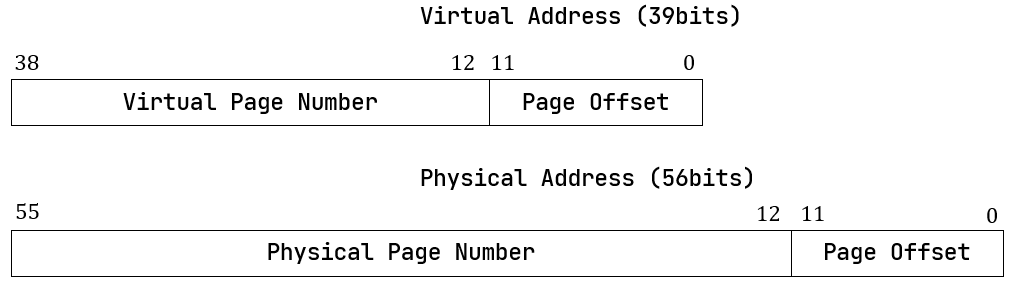
\includegraphics[width=0.8\linewidth]{figs/sv39-va-pa.png}
%       \caption{xxxx}
    \end{figure}
% 
% [sv39-va-pa](/Users/xyong/github/os-lectures/lecture04/figs/sv39-va-pa.png)
% 
% 
\end{frame}
%------------------------------------------------
\begin{frame}
    \frametitle{地址数据结构}
% %%%%%% 页表项
\href{https://github.com/rcore-os/rCore-Tutorial-v3/blob/ch4/os/src/mm/address.rs\#L5}{地址类型定义}:% struct PhysAddr、struct VirtAddr、struct PhysPageNum、struct VirtPageNum
    \begin{figure}
        \centering
        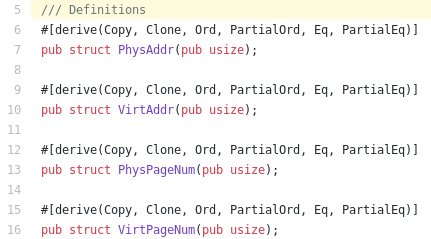
\includegraphics[width=0.4\linewidth]{figs/address-5.png}
%       \caption{xxxx}
    \end{figure}
% 
% [address-5](/Users/xyong/github/os-lectures/lecture04/figs/address-5.png)
% 
\href{https://github.com/rcore-os/rCore-Tutorial-v3/blob/ch4/os/src/mm/address.rs\#L88}{地址和页号的相互转换}:
    \begin{figure}
        \centering
        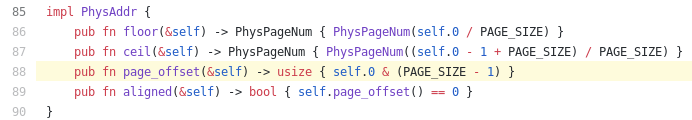
\includegraphics[width=0.7\linewidth]{figs/address-88.png}
%       \caption{xxxx}
    \end{figure}
% 
% [address-88](/Users/xyong/github/os-lectures/lecture04/figs/address-88.png)
% 
\end{frame}
%------------------------------------------------
\begin{frame}
    \frametitle{页表项的数据结构抽象与类型定义}
% %%%%%% 页表项
    \begin{figure}
        \centering
        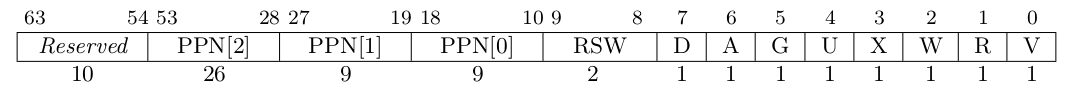
\includegraphics[width=0.6\linewidth]{figs/sv39-pte.png}
%       \caption{xxxx}
    \end{figure}
% 
% [sv39-pte](/Users/xyong/github/os-lectures/lecture04/figs/sv39-pte.png)
% 
% \href{https://rcore-os.github.io/rCore-Tutorial-Book-v3/chapter4/3sv39-implementation-1.html\#id5}{页表项的数据结构抽象与类型定义}
% 
\href{https://github.com/rcore-os/rCore-Tutorial-v3/blob/ch4/os/src/mm/page_table.rs\#L21}{PageTableEntry}
% 
% `PageTableEntry` 的工具\href{https://github.com/rcore-os/rCore-Tutorial-v3/blob/ch4/os/src/mm/page_table.rs\#L45}{函数}
    \begin{figure}
        \centering
        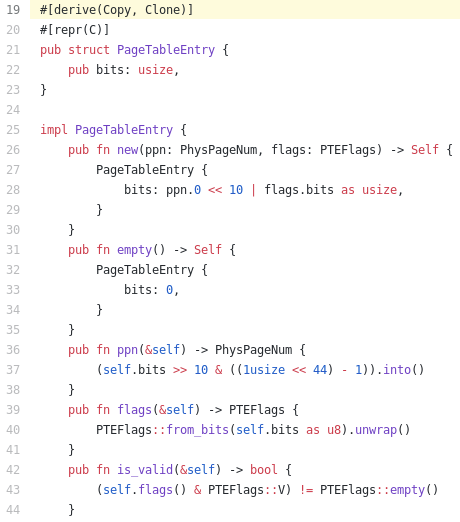
\includegraphics[width=0.6\linewidth]{figs/page_table-45.png}
%       \caption{xxxx}
    \end{figure}
% 
% [page_table-45](/Users/xyong/github/os-lectures/lecture04/figs/page_table-45.png)
% 
\end{frame}
%------------------------------------------------
\begin{frame}
    \frametitle{页表}
% %%%%%% 页表
% 
% \href{https://rcore-os.github.io/rCore-Tutorial-Book-v3/chapter4/4sv39-implementation-2.html\#id5}{多级页表实现}
% 
% `PageTable`\href{https://github.com/rcore-os/rCore-Tutorial-v3/blob/ch4/os/src/mm/page_table.rs\#L56}{数据结构}
    \begin{figure}
        \centering
        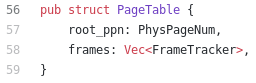
\includegraphics[width=0.6\linewidth]{figs/page_table-56.png}
%       \caption{xxxx}
    \end{figure}
% 
% [page_table-56](/Users/xyong/github/os-lectures/lecture04/figs/page_table-56.png)
% 
% \href{https://github.com/rcore-os/rCore-Tutorial-v3/blob/ch4/os/src/mm/page_table.rs\#L114}{PageTable}
% 
% 
\end{frame}
%------------------------------------------------
\begin{frame}
\frametitle{提纲} % Table of contents slide, comment this block out to remove it
\tableofcontents % Throughout your presentation, if you choose to use \section{} and \subsection{} commands, these will automatically be printed on this slide as an overview of your presentation
\end{frame}

%----------------------------------------------------------------------------------------

\subsection{地址转换}
\begin{frame}
    \frametitle{地址转换过程}
% %%%%%% 地址转换过程
% 
% \href{https://rcore-os.github.io/rCore-Tutorial-Book-v3/chapter4/3sv39-implementation-1.html\#id6}{多级页表原理}
% 
% SV39 地址转换的全过程
    \begin{figure}
        \centering
        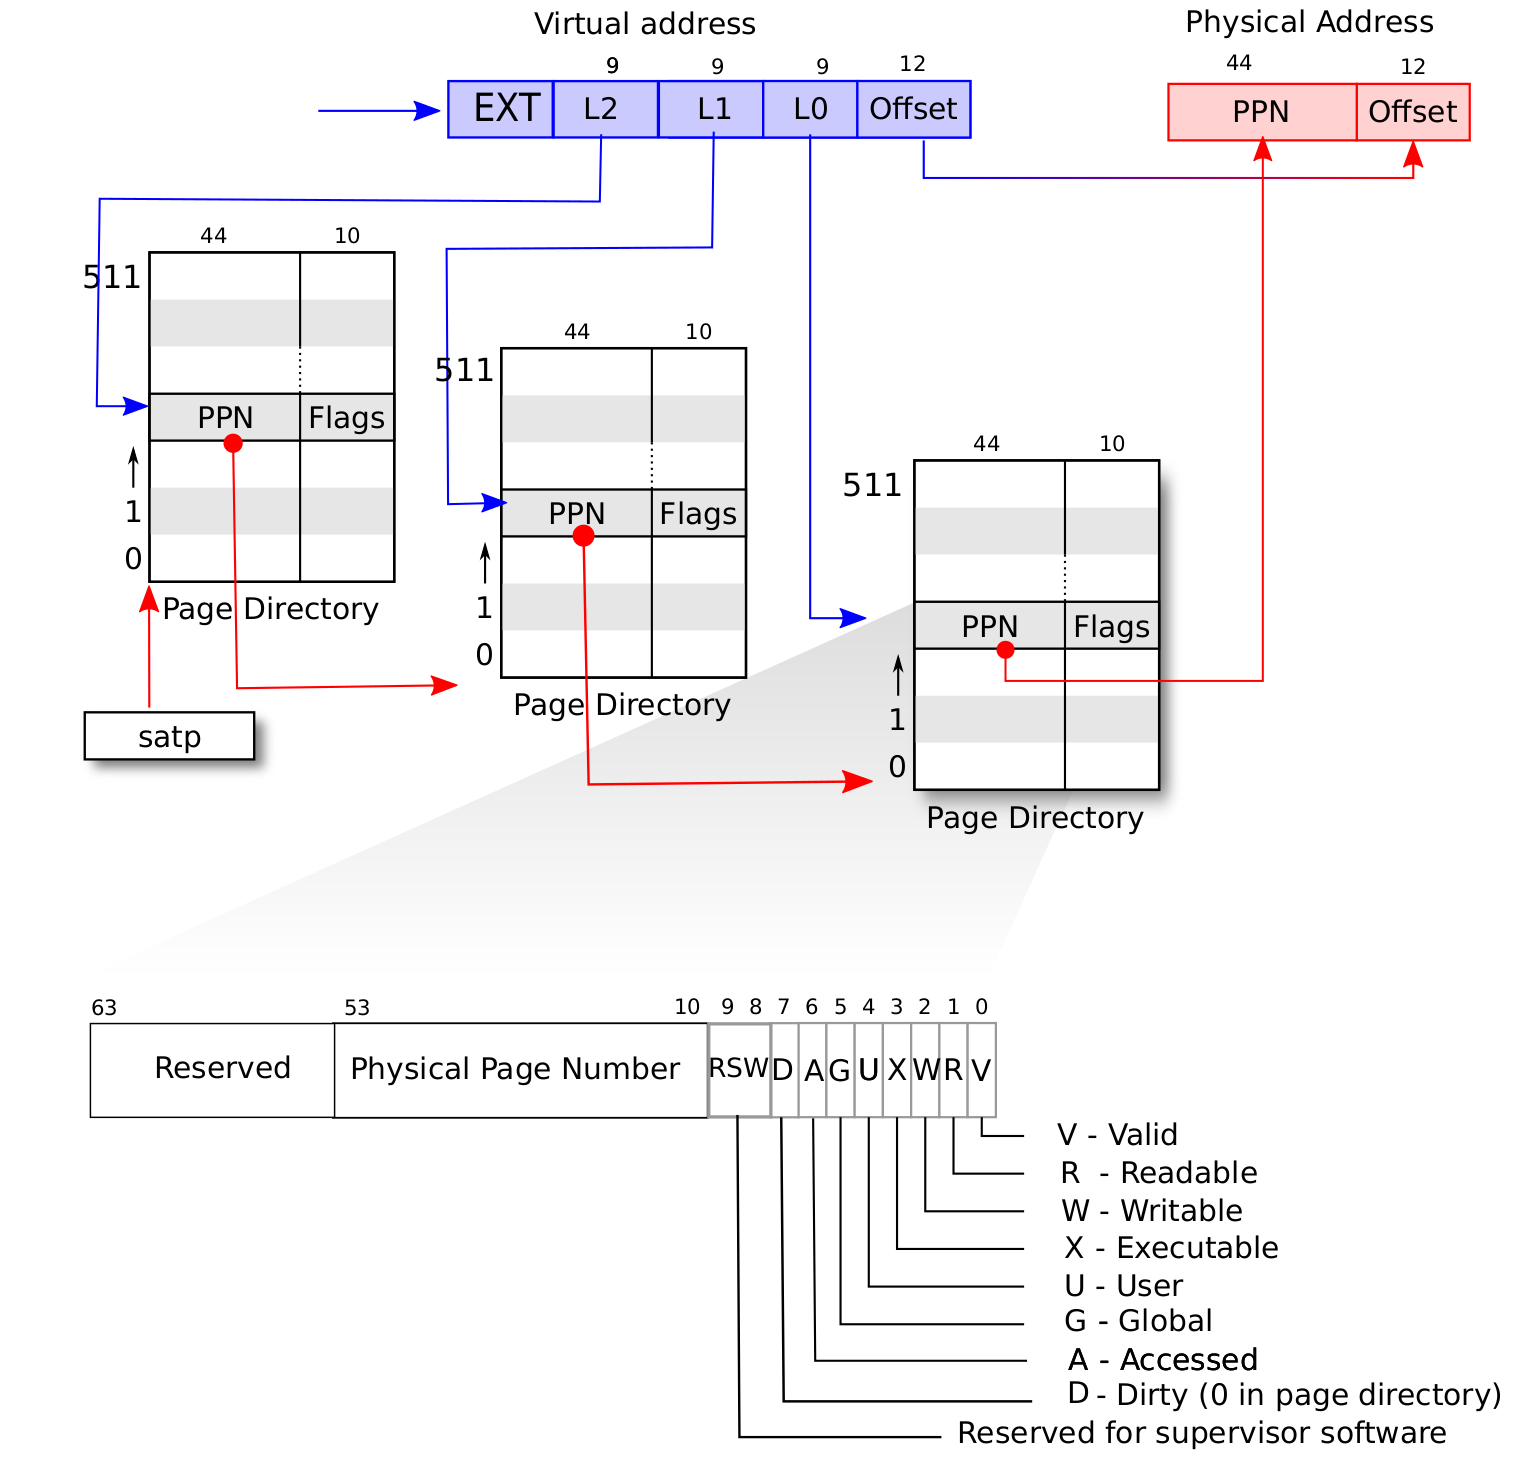
\includegraphics[width=0.45\linewidth]{figs/sv39-full.png}
%       \caption{xxxx}
    \end{figure}
% 
% [sv39-full](/Users/xyong/github/os-lectures/lecture04/figs/sv39-full.png)
% 
\end{frame}
%------------------------------------------------
\begin{frame}
    \frametitle{SV39 中的 R/W/X 组合的含义}
% SV39 中的 R/W/X 组合的含义
    \begin{figure}
        \centering
        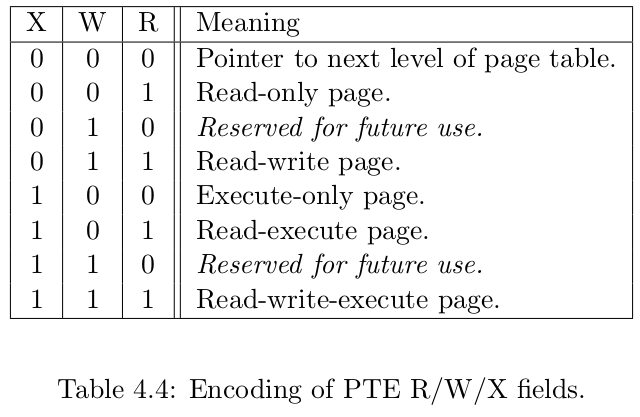
\includegraphics[width=0.6\linewidth]{figs/pte-rwx.png}
%       \caption{xxxx}
    \end{figure}
% 
% [pte-rwx](/Users/xyong/github/os-lectures/lecture04/figs/pte-rwx.png)
% 
% 
% 
\end{frame}
%------------------------------------------------
\begin{frame}
    \frametitle{地址映射建立和撤消}
% %%%%%% 地址映射建立和撤消
% 
% \href{https://rcore-os.github.io/rCore-Tutorial-Book-v3/chapter4/4sv39-implementation-2.html\#id8}{建立和拆除虚实地址映射关系}:
% 
        \begin{itemize}
        \item 在多级页表中找到一个虚拟地址对应的页表项
        \item 修改页表项的内容以建立虚实地址映射关系
        \item 页表中间的页表项可能未创建:手动分配物理页存放该页表项
        \end{itemize}
% 
% \href{https://github.com/rcore-os/rCore-Tutorial-v3/blob/ch4/os/src/mm/page_table.rs\#L114}{map}、\href{https://github.com/rcore-os/% rCore-Tutorial-v3/blob/ch4/os/src/mm/page_table.rs\#L120}{unmap}:
    \begin{figure}
        \centering
        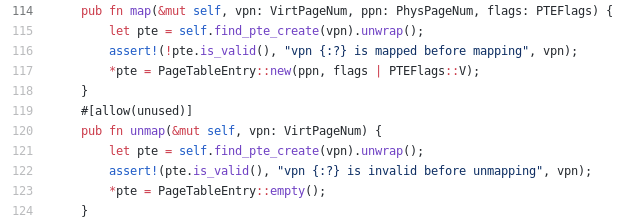
\includegraphics[width=0.8\linewidth]{figs/page_table-114.png}
%       \caption{xxxx}
    \end{figure}
% 
% [page_table-114](/Users/xyong/github/os-lectures/lecture04/figs/page_table-114.png)
% 
% 
% 
\end{frame}
%------------------------------------------------
\begin{frame}
    \frametitle{物理页管理}
% %%%%%% 物理页管理
% 
% \href{https://rcore-os.github.io/% rCore-Tutorial-Book-v3/chapter4/4sv39-implementation-2.html\#sv39}{实现 SV39 多级页表机制(下)}:物理内存管理、多级页表、地址转换;
% 
% \href{https://rcore-os.github.io/rCore-Tutorial-Book-v3/chapter4/4sv39-implementation-2.html\#id2}{物理页帧管理}:
% 
        \begin{itemize}
        \item 声明一个 `FrameAllocator` Trait 描述物理页帧管理器的功能
        \item 实现一种简单的栈式物理页帧管理策略 `StackFrameAllocator` 
        \end{itemize}
% 
% \href{https://github.com/rcore-os/rCore-Tutorial-v3/blob/ch4/os/src/mm/frame_allocator.rs\#L35}{FrameAllocator}
    \begin{figure}
        \centering
        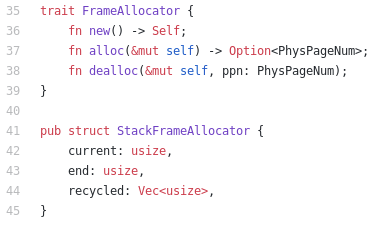
\includegraphics[width=0.6\linewidth]{figs/frame_allocator-L35.png}
%       \caption{xxxx}
    \end{figure}
% 
% [frame_allocator-L35](/Users/xyong/github/os-lectures/lecture04/figs/frame_allocator-L35.png)
% 
\end{frame}
%------------------------------------------------
\begin{frame}
    \frametitle{栈式物理页帧管理策略}
% 栈式物理页帧管理策略
% 
        \begin{itemize}
        \item 分配 `alloc` 时,检查栈 `recycled` 内有没有之前回收的物理页号;
            \begin{itemize}
            \item 如果有的话直接弹出栈顶并返回;
            \item 否则,从之前从未分配过的物理页号区间的左端点 `current`分配。
            \end{itemize}
        \item 回收 `dealloc` 时,检查回收页面的合法性,然后将其压入 `recycled` 栈中。
        \end{itemize}
% 
% 
% 
% 
\end{frame}
%------------------------------------------------
\begin{frame}
\frametitle{提纲} % Table of contents slide, comment this block out to remove it
\tableofcontents % Throughout your presentation, if you choose to use \section{} and \subsection{} commands, these will automatically be printed on this slide as an overview of your presentation
\end{frame}

%----------------------------------------------------------------------------------------
\subsection{地址空间}
\begin{frame}
    \frametitle{地址空间与段}
% %%%%%% 地址空间与段
% 
\href{https://rcore-os.github.io/rCore-Tutorial-Book-v3/chapter4/5kernel-app-spaces.html\#id4}{逻辑段}:指地址区间中的一段属性相同的连续虚拟地址区间,以相同方式映射到物理页帧。
% 
% \href{https://github.com/rcore-os/rCore-Tutorial-v3/blob/ch4/os/src/mm/memory_set.rs\#L193}{MapArea}
    \begin{figure}
        \centering
        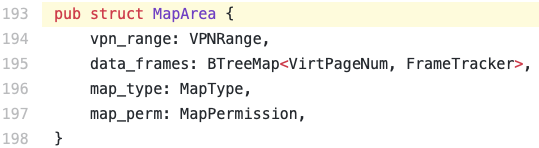
\includegraphics[width=0.6\linewidth]{figs/memory_set-L193.png}
%       \caption{xxxx}
    \end{figure}
% 
% [memory_set-L193](/Users/xyong/github/os-lectures/lecture04/figs/memory_set-L193.png)
% 
\href{https://rcore-os.github.io/rCore-Tutorial-Book-v3/chapter4/5kernel-app-spaces.html\#id5}{地址空间}:包含一个多级页表page\_table 和一个逻辑段MapArea的向量areas
% 
% \href{https://github.com/rcore-os/rCore-Tutorial-v3/blob/ch4/os/src/mm/memory_set.rs\#L38}{struct MemorySet}
    \begin{figure}
        \centering
        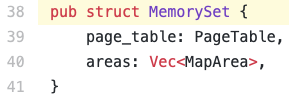
\includegraphics[width=0.4\linewidth]{figs/memory_set-L38.png}
%       \caption{xxxx}
    \end{figure}
% 
% [memory_set-L38](/Users/xyong/github/os-lectures/lecture04/figs/memory_set-L38.png)
% 
% 注:\href{https://www.tomdalling.com/blog/software-design/% resource-acquisition-is-initialisation-raii-explained/}{Resource Acquisition is Initialisation (RAII) Explained}
% 
\end{frame}
%------------------------------------------------
\begin{frame}
    \frametitle{\href{https://rcore-os.github.io/rCore-Tutorial-Book-v3/_images/kernel-as-high.png}{内核地址空间高256GiB布局}}
% %%%%%% 内核地址空间
% 
% \href{https://rcore-os.github.io/rCore-Tutorial-Book-v3/chapter4/5kernel-app-spaces.html\#id6}{内核地址空间}
% 
% \href{https://rcore-os.github.io/rCore-Tutorial-Book-v3/_images/kernel-as-high.png}{内核地址空间高256GiB布局}
    \begin{figure}
        \centering
        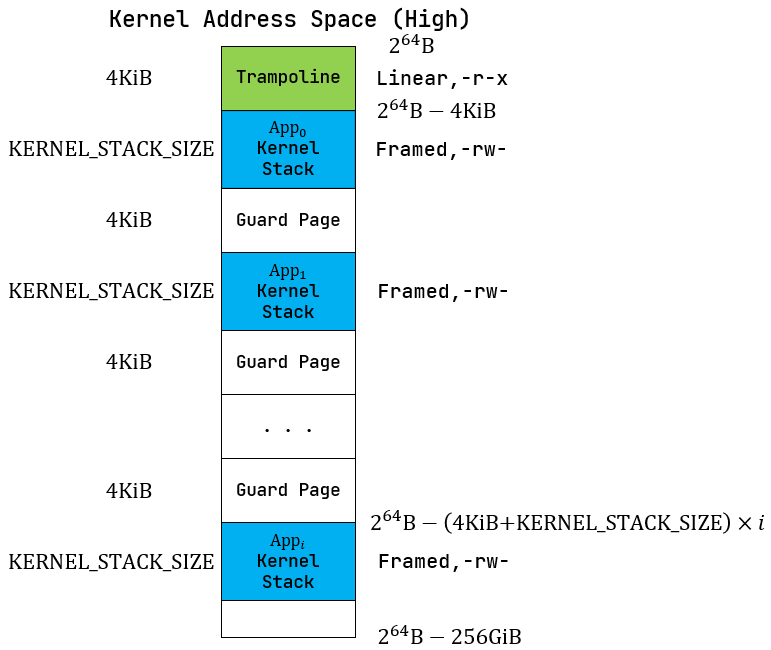
\includegraphics[width=0.5\linewidth]{figs/kernel-as-high.png}
%       \caption{xxxx}
    \end{figure}
% 
% [kernel-as-high](/Users/xyong/github/os-lectures/lecture04/figs/kernel-as-high.png)
% 
\end{frame}
%------------------------------------------------
\begin{frame}
    \frametitle{\href{https://rcore-os.github.io/rCore-Tutorial-Book-v3/_images/kernel-as-low.png}{内核地址空间低256GiB布局}}
四个逻辑段 .text/.rodata/.data/.bss 被恒等映射到物理内存;
    \begin{figure}
        \centering
        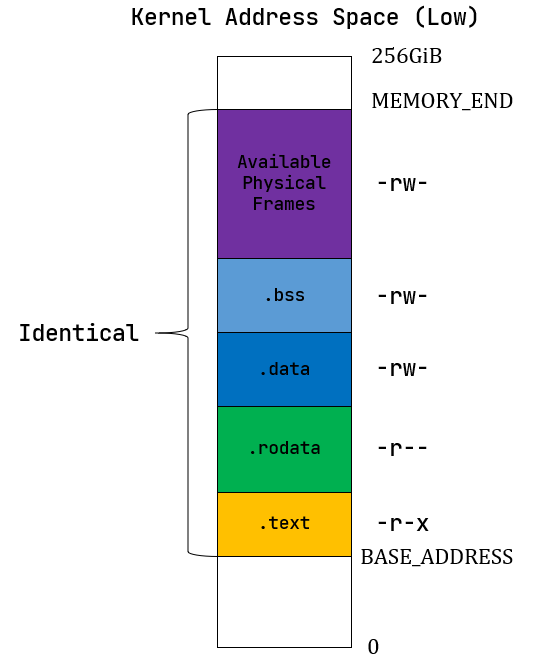
\includegraphics[width=0.35\linewidth]{figs/kernel-as-low.png}
%       \caption{xxxx}
    \end{figure}
% 
% [kernel-as-low](/Users/xyong/github/os-lectures/lecture04/figs/kernel-as-low.png)
% 
% 
% 
% 
% 
% \href{https://github.com/rcore-os/rCore-Tutorial-v3/blob/ch4/os/src/mm/memory_set.rs\#L78}{new_kernel}
% 
% 保护页面 (Guard Page)
% 
\end{frame}
%------------------------------------------------
\begin{frame}
    \frametitle{\href{https://rcore-os.github.io/rCore-Tutorial-Book-v3/chapter4/5kernel-app-spaces.html\#id7}{应用地址空间}}
% %%%%%% 用户地址空间 
% 
借助地址空间的抽象,可以让所有应用程序都使用同样的起始地址;
% 
% \href{https://rcore-os.github.io/rCore-Tutorial-Book-v3/_images/app-as-full.png}{应用地址空间的布局}
    \begin{figure}
        \centering
        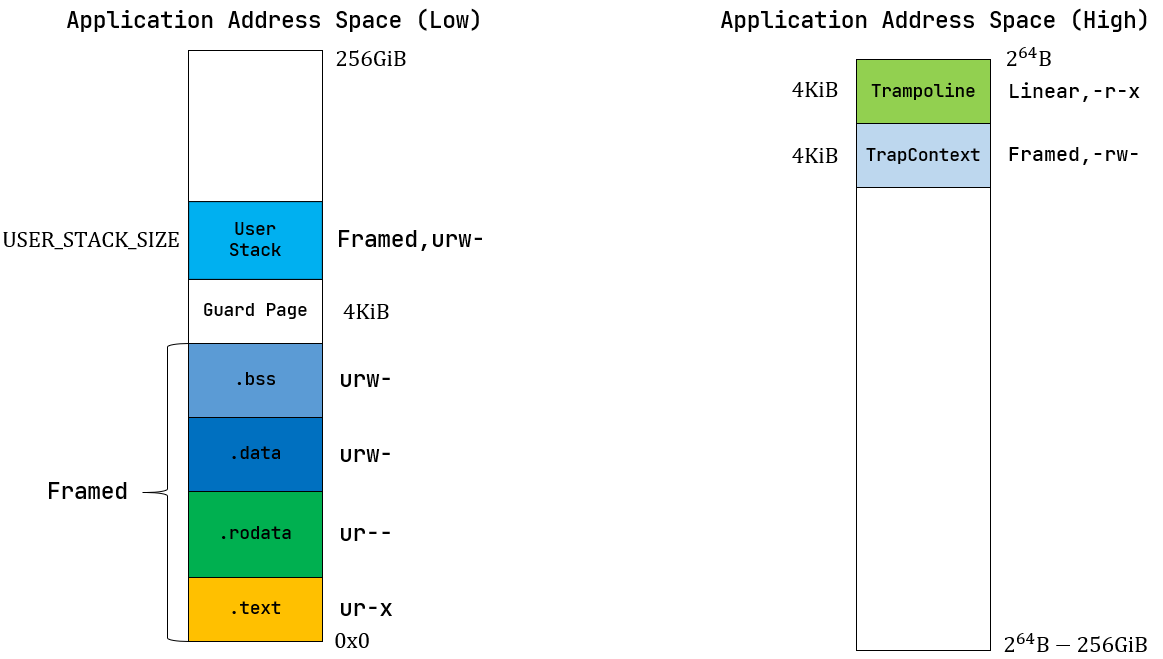
\includegraphics[width=0.6\linewidth]{figs/app-as-full.png}
%       \caption{xxxx}
    \end{figure}
% 
% [app-as-full](/Users/xyong/github/os-lectures/lecture04/figs/app-as-full.png)
% 
% \href{https://github.com/rcore-os/rCore-Tutorial-v3/blob/ch4/os/src/mm/memory_set.rs\#L126}{from_elf}
% 
\end{frame}
%------------------------------------------------
\begin{frame}
    \frametitle{内核地址空间初始化}
% %%%%%% 内核地址空间初始化
% 
% \href{https://rcore-os.github.io/rCore-Tutorial-Book-v3/chapter4/6multitasking-based-on-as.html\#id1}{建立并开启基于分页模式的虚拟地址空间}
% 
        \begin{itemize}
        \item CPU 将跳转到内核入口点并在 S 特权级上执行,此时并没有开启分页模式;
        \end{itemize}
% 
\href{https://github.com/rcore-os/rCore-Tutorial-v3/blob/ch4/os/src/mm/mod.rs\#L15}{内核地址空间初始化}
    \begin{figure}
        \centering
        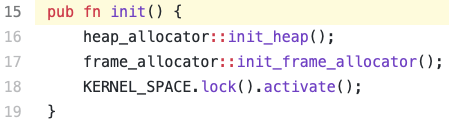
\includegraphics[width=0.6\linewidth]{figs/mod-L15.png}
%       \caption{xxxx}
    \end{figure}
% 
% [mod-L15](/Users/xyong/github/os-lectures/lecture04/figs/mod-L15.png)
% 
\end{frame}
%------------------------------------------------
\begin{frame}
    \frametitle{使能分页机制}
% %%%%%% 使能分页机制
% 
% [SV39 分页模式启用]():S特权级的MMU使能;
% 
        \begin{itemize}
        \item 切换 satp CSR 必须是平滑,即切换 satp 的指令及其下一条指令的虚拟地址是相邻的;
        \item 内核内存布局的代码段在切换之后采用恒等映射,切换前的物理地址直接访问可视为恒等映射。
        \end{itemize}
% 

% 
\end{frame}

\begin{frame}
\frametitle{提纲} % Table of contents slide, comment this block out to remove it
\tableofcontents % Throughout your presentation, if you choose to use \section{} and \subsection{} commands, these will automatically be printed on this slide as an overview of your presentation
\end{frame}
\subsection{地址空间切换}

%----------------------------------------------------------------------------------------

%------------------------------------------------
\begin{frame}
    \frametitle{用户态与内核态间的地址空间切换:\href{https://rcore-os.github.io/rCore-Tutorial-Book-v3/chapter4/6multitasking-based-on-as.html\#id6}{跳板的实现}}
% %%%%%% 用户态与内核态间的地址空间切换
% 

% 
需求:
% 
        \begin{itemize}
        \item 使能了分页机制后,必须用户态与内核态切换中同时完成地址空间的切换。
        \item 通过修改 satp 在应用地址空间和内核地址空间间切换。
        \item 应用和内核地址空间在切换地址空间指令附近是平滑的。
        \end{itemize} \pause
% 
实现:
% 
        \begin{itemize}
        \item 内核与用户进程各有自己的地址空间,共享同一个Trampoline( \_\_alltraps 的代码)和TrapContext( \_\_alltraps 的数据);Trampoline可在用户地址空间和内核态时访问。
        \item 当应用 Trap 进入内核时,硬件会设置一些 CSR 并在 S 特权级下跳转到 \_\_alltraps 保存 Trap 上下文。
        \end{itemize}
% 
\end{frame}
%------------------------------------------------
\begin{frame}
    \frametitle{建立跳板}
% %%%%%% 建立跳板
% 
map\_trampoline建立跳板区域的虚实映射关系:
% 
        \begin{itemize}
        \item 用户态是不能访问的;
        \item 中断时,中断进入时硬件保存现场并不直接访问这个区域的内存,而是放在寄存器中;
        \item 这个区域只在内核态且是用户地址空间时访问;
        \item 这两个页表的设置是一样的,可以保证它只在内核态可以访问;
        \item 中断服务例程的地址在链接时得到;
        \end{itemize}
\end{frame}
%------------------------------------------------

%----------------------------------------------------------------------------------------

\end{document}
